\section{Wykonywanie eksperymentów}
\label{podzial_zadan}

\begin{frame}
    \frametitle{Eksperymenty}
    
    \begin{figure}[H]
    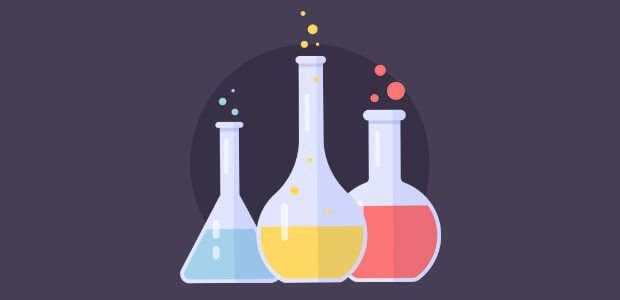
\includegraphics[scale=0.5]{img/exp1.jpg} 
    \end{figure}
    
\end{frame}

\begin{frame}
    \frametitle{Przygotowanie scenariuszy testowych}
    \begin{figure}[!tbp]
      \centering
      \begin{minipage}[b]{0.4\textwidth}
        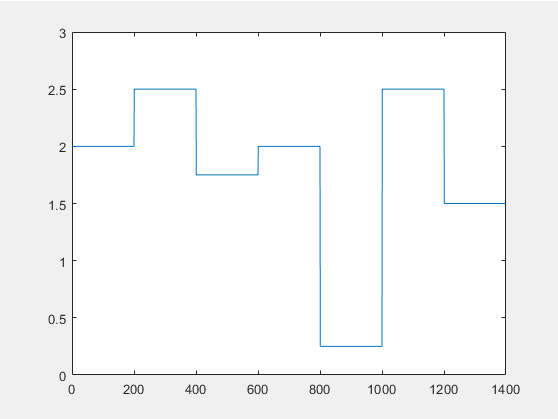
\includegraphics[scale = 0.35]{img/dobry_przebieg.PNG}
        \caption*{Dobry przebieg}
      \end{minipage}
      \hfill
      \begin{minipage}[b]{0.4\textwidth}
        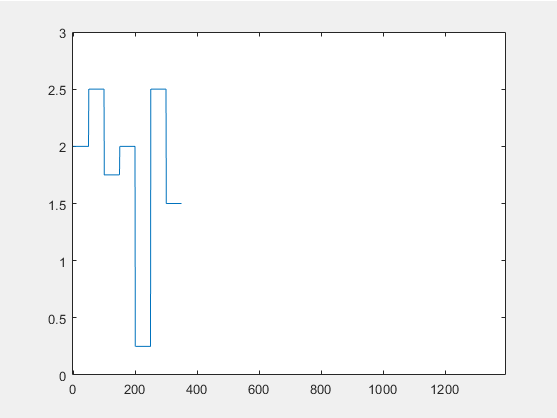
\includegraphics[scale = 0.35]{img/zly_przebieg.PNG}
        \caption*{Zły przebieg}
      \end{minipage}
    \end{figure}
\end{frame}

\begin{frame}
    \frametitle{Zautomatyzowanie testowania}
    \begin{figure}[H]
    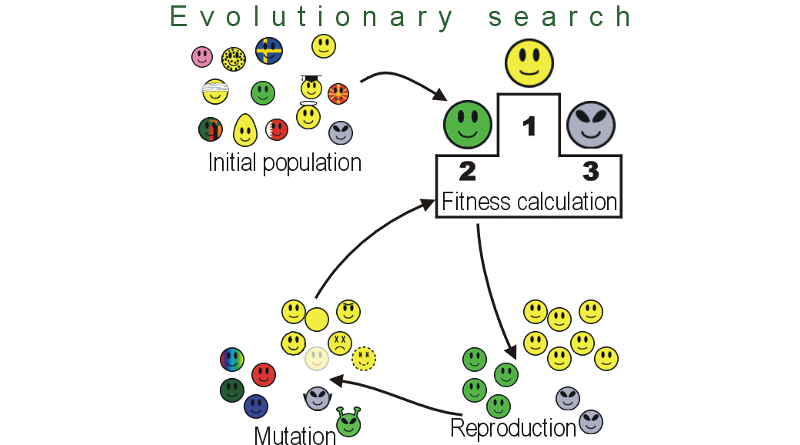
\includegraphics[scale=1.8]{img/algorytm_ewolucyjny.png} 
    \end{figure}
\end{frame}

\begin{frame}
    \frametitle{Przygotowanie się na potencjalne błędy podczas testowania}
    \begin{figure}[H]
    
\includegraphics[scale=0.3]{img/error.jpg} 
    \end{figure}
\end{frame}

\begin{frame}
    \frametitle{Podsumowanie części związanej z eksperymentami}
    \begin{figure}[H]
    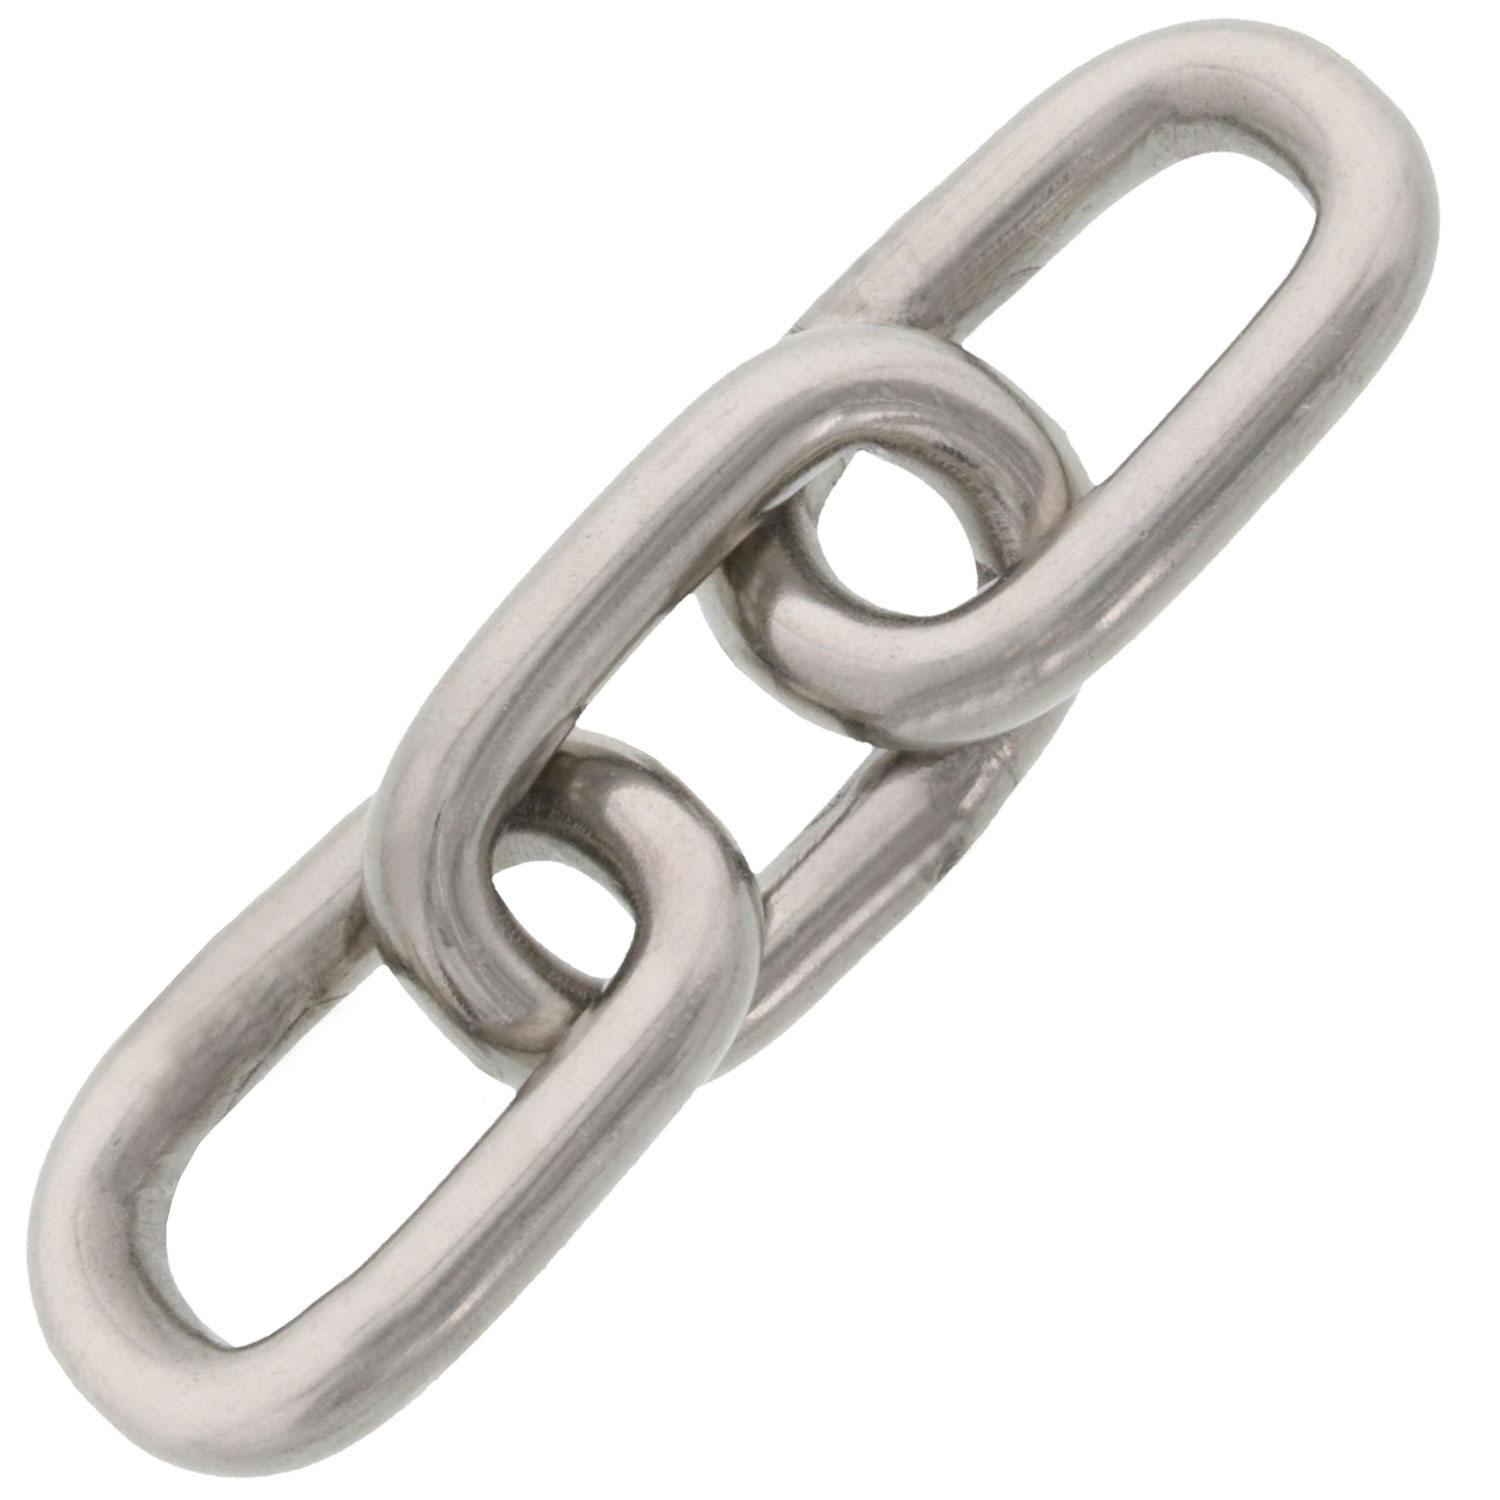
\includegraphics[scale=0.13]{img/chain.jpg} 
    \end{figure}
\end{frame}